\section{The Social Continuum of Sharing Surrounding Spaces in Wearable AR}

% \subsection{Abstract}

This paper describes a system and a user study for sharing social surrounding spaces on wearable Augmented Reality (AR) devices. Unlike sharing for collaborative purposes, we focus on sharing between social contacts. We extend the previous work of the Social AR Continuum by exploring how sharing the surrounding environment can vary based on the social proximity between social contacts. We built a prototype for sharing a 3D captured room on a HoloLens, which enables the user to display three levels of social relationships: intimate, friend and stranger and maps them to three levels of the surrounding environment. In a user study with the prototype, we focused on how socially connected participants felt, as well as on how they felt knowing that they were sharing more or fewer details of their surrounding environment with their social contacts. We found that all participant preferred having a social filter when sharing a view of their environment over having no filter. We discuss the research findings and outline future directions for research in sharing social surrounding spaces on wearable AR devices. 
 

% Wearable Augmented Reality (AR) devices are becoming more affordable, available and ubiquitous, so there is a need to understand design considerations for this new platform. Previous research has looked into using wearable AR headsets for collaborative use, for example in enhancing face to face \cite{Billinghurst2002} or remote collaboration \cite{gupta2016you}. The research presented here explores the use of AR headsets for social interaction and shared experiences. 

% Future social interactions with wearable AR can be extrapolated from current social network interactions where friends share content and interact with others' content on mobile platforms such as Facebook and Instagram. One trend with mobile social networks is live streaming of a view of a user’s surroundings. For example, Facebook live allows a person with a mobile phone to live stream to remote collaborators. Similarly, wearable AR systems have already been developed that enable people to share a view of their surroundings. For example, the Shared Sphere work of \cite{lee2017mixed} allows a user with a wearable AR display to live stream a 360 video of their surroundings to a remote collaborator. 

It is easy to imagine that in the future it will be possible for wearable AR systems to be used to capture and share a 3D view of the user's surroundings with hundreds or thousands of followers on a social network. However, before this becomes commonplace, many exciting research questions should be addressed. For example, would a person be comfortable with sharing a view of their real space with relative strangers? This work aims to explore how wearable AR systems could share a user’s surrounding room environment with social contacts and to measure how comfortable the sharer and the viewer would feel regarding privacy in different interface options. 

In the remainder of the paper, we first report on related work that is informing our research, then describe a prototype system we have developed mocking up potential interface options. In sections 4 and 5 we present the design of a user study with the prototype and in sections 6 and 7 the results of the study. Finally, we end the paper with a conclusion and discussion of areas for future research.


% \subsection{Background}

% Our work extends earlier work in representing users in Augmented and Virtual Reality (VR), social networking, and AR information filtering. Previous researchers have studied the concept of "personal space" and "social bubbles" as proxemic interactions between people in different places \cite{Sousa2016}. They used floor projections and hand-held devices to communicate the presence of remote people. They also established a "gradual engagement model for remote proxemics" based on distance from the user which consists of 1) personal, 2) engaged, 3) peripheral and 4) ambient.

% \cite{Jo2016} studied the influence on co-presence of the background environment (AR vs VR) and the fidelity of the avatar representation of the remote user (photo-realistic vs pre-built). They found that more realistic avatars had a positive impact on the feeling of co-presence between remote collaborators. \cite{Volante2016} also studied the impact of the visual appearance of avatars (realistic vs. stylized) on the inter-personal emotional response of participants. 

% \cite{Fuchs2014} studied telepresence via a scanned 3D environment to enable social connections with people and simulated face-to-face interactions. The remote person was scanned and reconstructed live in the local environment. They forecast that 3D telepresence is going to be more popular when technology is more capable. Similarly, some companies (such as High Fidelity and Itsme3D) are building social VR experiences in which users are represented as 3D virtual avatars.

% Although there has been considerable research into social representation in VR, there has been very little research in AR. There are some challenges with AR, such as finding the best locations to fit virtual avatars in the real world, so they do not interfere with physical objects or appear suspended in mid-air. However, a social AR application can also allow people to see their friends while doing other tasks; users do not have to switch to an immersive VR environment to see their social contacts.

% If AR is to be used to represent contacts in social networks, there could be a large number of contact to show. So our research could also benefit from earlier work on different ways of managing large amounts of information in AR interfaces. \cite{Julier2002} showed how environmental cues such as distance, and user context could be used to filter AR content into the most relevant information. View management techniques can be used to ensure that virtual objects can be easily seen in collaborative AR interfaces \cite{Hollerer2001}. Similarly, an image-based can be used to ensure AR information tags do not overlap in the AR view \cite{Grasset2012}. 

% In some mobile AR applications, the technology can be used to share a view of the user's world. For example, remote collaboration systems have been developed where a local worker with an AR display can share a live video view of their working space with a remote expert \cite{Billinghurst2002}, and the remote expert can provide visual feedback with AR graphical cues. However, most of these systems have just been developed for collaboration between small numbers of users, and not for more extensive social networks.

% Compared to this earlier research our work is novel because it considers how a wearable AR interface could be used to share views of a user’s surroundings with a vast social network with people of different relationships. When connected in this way, people may want to control the amount of information about their surroundings shared. For example, users who are close friends in a social network may be happy to share a view of their surroundings and have the remote user appear as an AR avatar in their real space, while those that are strangers may only prefer to have an audio connection and not show anything of their surroundings to preserve their privacy \cite{Oetzel2011}.

% We extend our previous research of the social AR continuum \cite{Nassani2017a} that describe parameters/dimensions that can be used for sharing social experiences. Previously, we investigated visual representation of virtual avatars on social AR in \cite{Nassani2017b} where we filter representing social contacts (intimate, friend, acquaintance and stranger) based on social proximity. We also looked into filtering social data (360 video, 2D video and 2D image) in \cite{Nassani2018a} as well as filtering the surrounding environment (full, half and limited room) in \cite{Nassani2018b} based on social proximity. In this work (Figure \ref{fig:frontier18:social-filter}), we focus the feeling of privacy when sharing and viewing surrounding spaces as well as the hiding mechanism preferred by users. 

\begin{figure}
\begin{center}
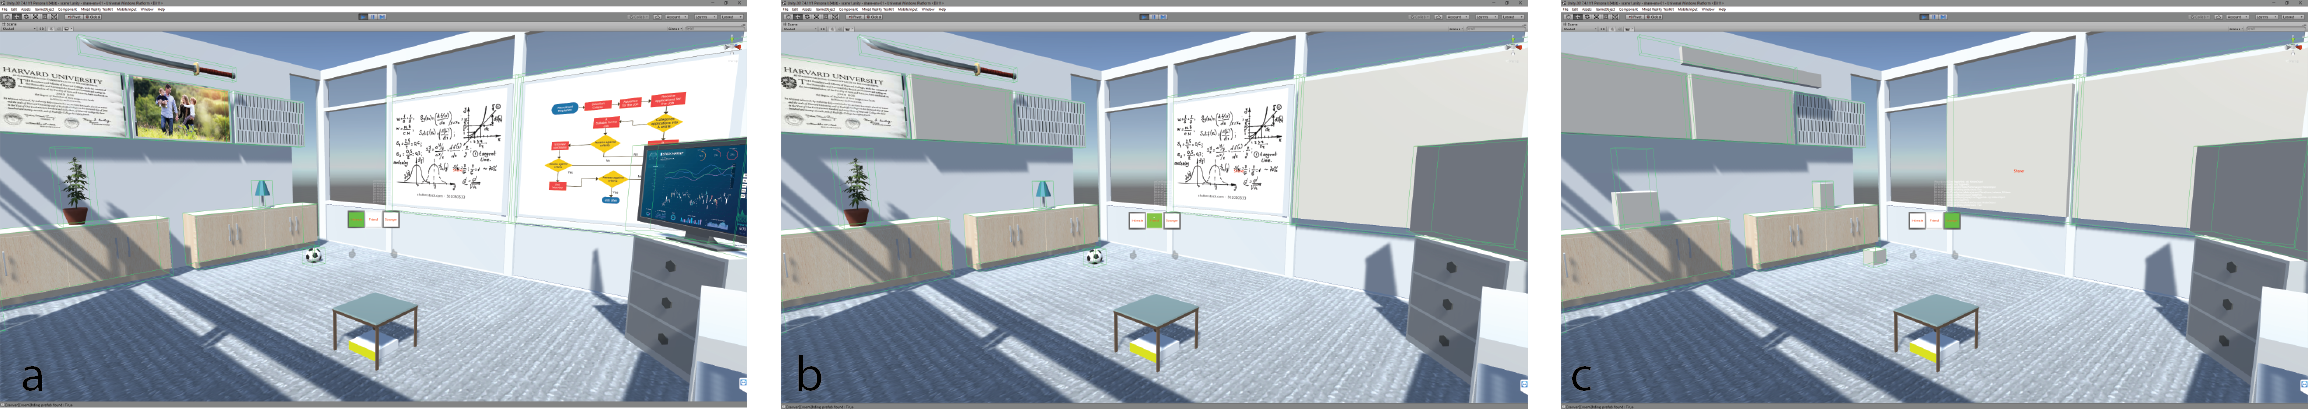
\includegraphics[width=\linewidth]{images/frontier18/images-02.png}
\caption{Social filter applied to the shared room. a) In an Intimate relationship, everything is shared. b) For a Friend relationship, some sensitive items are hidden (e.g., family photo, stock market). c) While for a Stranger relationship almost everything is hidden in the room.}\label{fig:frontier18:social-filter}
\end{center}
\end{figure}

\subsection{System}


We built an AR prototype system on the Microsoft HoloLens\footnote{https://www.microsoft.com/en-us/hololens} that connects a person (the sharer) sharing a view of their surrounding physical space to a remote person (the viewer) viewing the shared virtual room overlaid on top of their physical space. Figure \ref{fig:frontier18:system} shows the components of the system that we developed.

In the future, it will be possible to scan and immediately create a 3D model of the wearable AR user’s surroundings. However, we emulate this by creating a virtual 3D room modelled to match the sharer’s real room as if has been 3D scanned (see figure 2).  The 3D modelling was done on Autodesk Maya\footnote{https://www.autodesk.com/education/free-software/maya} and rendered on the HoloLens display using the Unity3D\footnote{https://unity3d.com/} game engine. The avatars representing the remote people are generated using MakeHuman\footnote{http://www.makehumancommunity.org/}.

We used UNET\footnote{https://docs.unity3d.com/Manual/UNet.html} as the high-level networking API from Unity to synchronise the state of the shared room and the remote person. The state of the remote person includes 1) the position and rotation of the virtual avatar representing the remote person, 2) the level of detail of the avatar based on the social relationship (i.e., stranger=half 2D image, friend=2D image, intimate=3D avatar). The synchronised state of the room involves changing the level of detail of the shared room depending on the social relationship as well as which part of the room is hidden by the user. 

\begin{figure}
\begin{center}
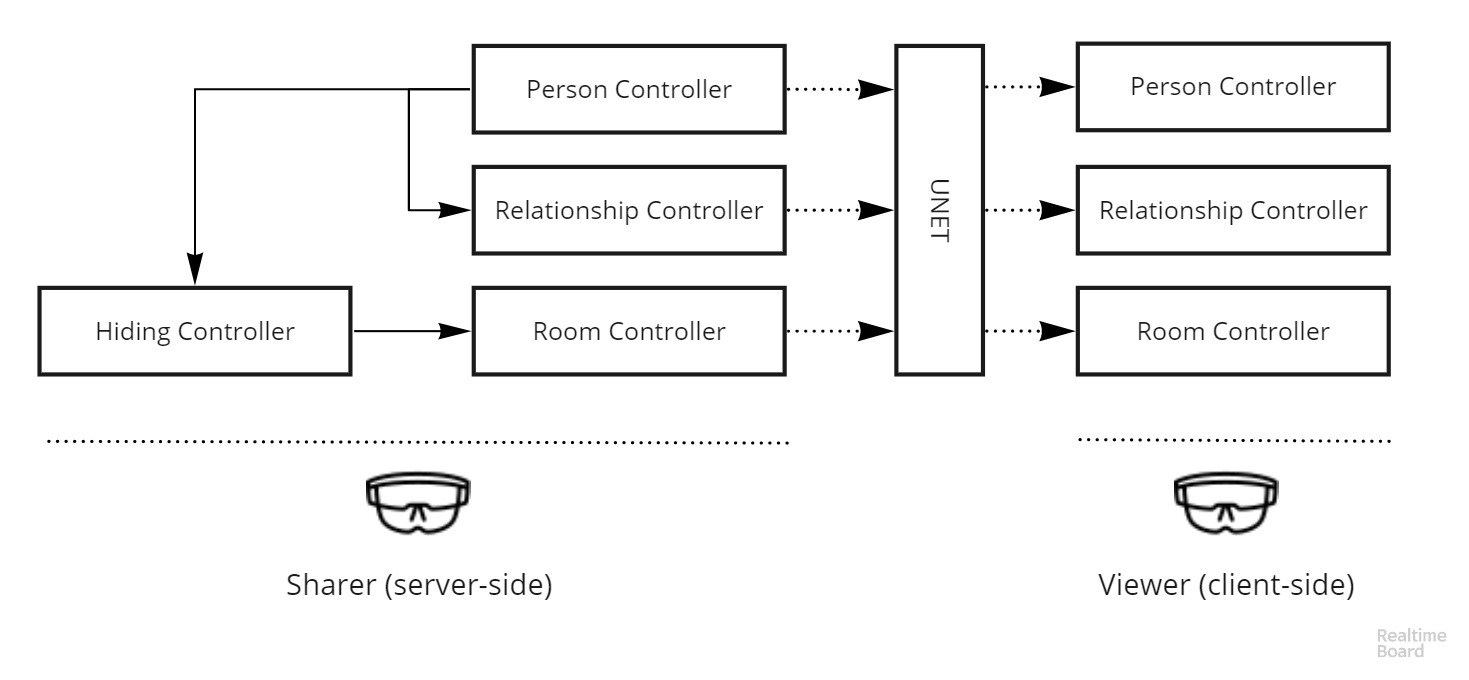
\includegraphics[width=\linewidth]{images/frontier18/system.jpg}
\caption{System components representing the sharer server-side (left) sharing with the viewer client-side (right) via WiFi: 1) the avatar position and orientation, 2) the social relationship data and 3) room and hidden components data. The system is built on Unity and runs on HoloLens.}\label{fig:frontier18:system}
\end{center}
\end{figure}

\subsection{User Study}

Using the prototype system we wanted to explore sharing different views depending on the social relationship between users, and also different methods for maintaining privacy. To do this, we conducted a pilot user study, with 12 participants (4 female) aged (25 – 43, median=32, SD=4.96). 
We asked participants to do two tasks: 

Task 1: View/share a room with or without a social proximity filter (see Figure \ref{fig:frontier18:social-filter}). In this task we had two conditions: 

\begin{itemize}
\item T1C1: Shared room without a social proximity filter where the level of details of the shared room is not affected by the social relationship between the users.
\item T1C2: Shared room with a social proximity filter where the level of details of the shared room is changed based on the social relationship between the users. 
\end{itemize}

Task 2:  The mechanism of hiding room parts for social proximity filter (see Figure \ref{fig:frontier18:hiding-mechanism}). In this task we had three conditions:

\begin{itemize}
\item T2C1: Remove – where objects are hidden by being removed from the viewer’s scene.
\item T2C2: Overlay – where objects are hidden by being overlaid by a white box. 
\item T2C3: Blur – where objects are hidden by appearing blurred to the viewer. 
\end{itemize}

Each participant tried the conditions from both sides of a viewer and a sharer. We asked participants to rate their experience after each condition. At the end of each task, we asked them to compare the conditions to each other and rank them. 

\begin{figure}
\begin{center}
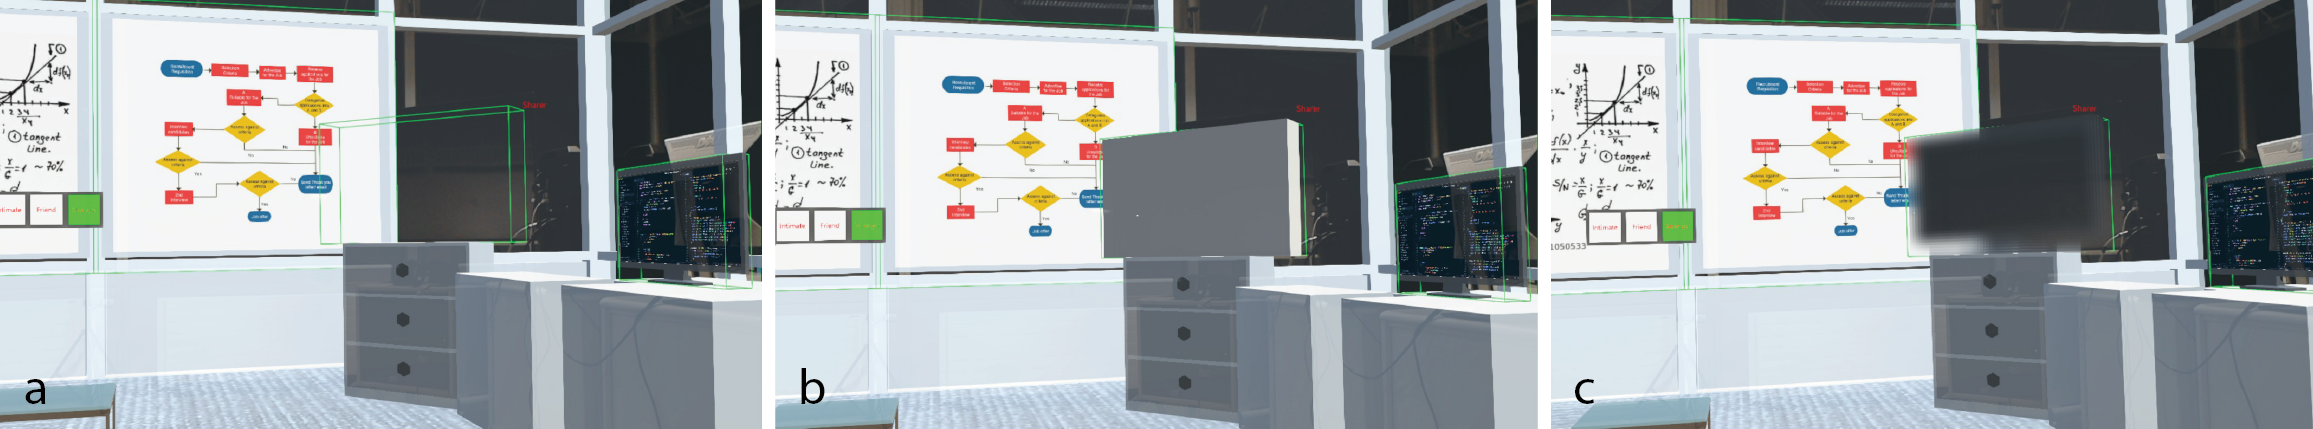
\includegraphics[width=\linewidth]{images/frontier18/images-01.png}
\caption{Hiding mechanism applied on the TV screen. a) Remove, b) Overlay, c) Blur.}\label{fig:frontier18:hiding-mechanism}
\end{center}
\end{figure}


% \subsection{Experiment}

Figure \ref{fig:frontier18:setup} shows that the experiment was set up in two similar rooms so that the sharer was sharing his/her room with a remote viewer. The relative position and rotation of each user were synchronised and represented as a virtual avatar in the remote person view. The sharer could change the social relationship with the viewer by using 3-buttons (intimate, friend, stranger) situated in the middle of the room. The viewer could request the relationship to change by clicking on one of the relationship buttons. Once this happens, the sharer saw the relationship request in a different colour, which then they could approve and change the social relationship

After completing each task, we asked participants (see Table \ref{tab:frontier18:questions}) to answer three sets of Likert questionnaires; six bi-polar questions (BP), six co-presence questions (CoP) and three subjective questions (S) to measure the sense of privacy.  

\begin{table}
    \centering
    \begin{tabular}{ll}
BP1 &    Impersonal-Personal\\
BP2 &    Cold-Warm\\
BP3 &    Colourless-Colourful\\
BP4 &    Unsociable-Sociable\\
BP5 &    Closed-Open\\
BP6 &    Passive-Active\\
CoP1    &   I noticed my partner\\
CoP2    &   My partner noticed me\\
CoP3    &   My partner's presence was obvious to me\\
CoP4    &   My presence was obvious to my partner\\
CoP5    &   My partner caught my attention \\
CoP6    &   I caught my partner's attention\\
S1  & Uncomfortable-Comfortable\\
S2  & Insecure-Secure\\
S3  & Not-Interested-Interested\\
    \end{tabular}
    \caption{Subjective questions we asked participants to rate their experience on a 7-point likert scale}
    \label{tab:frontier18:questions}
\end{table}

We asked the participants open-ended questions about the strength and weakness of each condition. We also asked them to rank from most preferred to least preferred condition for each task, then explain the reason for why the chose the best and the worst condition. 

\begin{figure}
\begin{center}
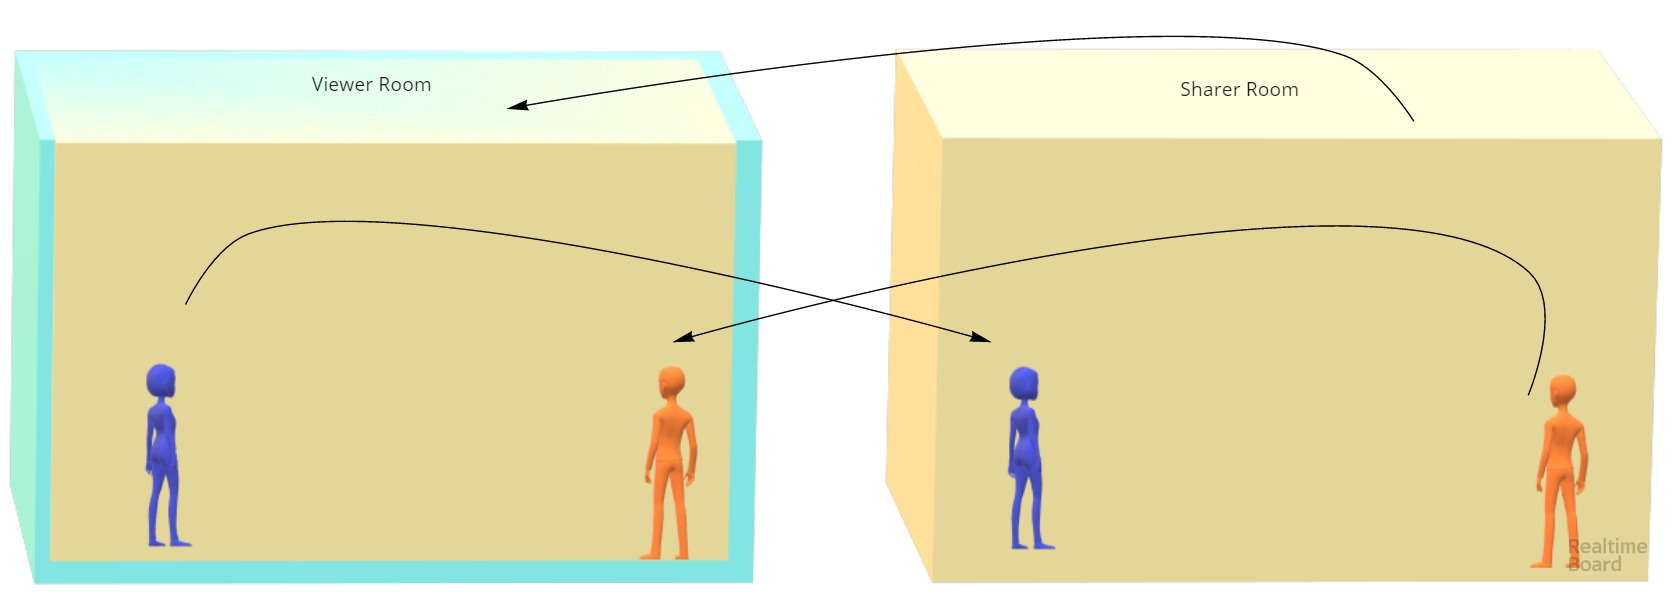
\includegraphics[width=\linewidth]{images/frontier18/experiment-setup.jpg}
\caption{Experiment setup. The sharer (right) is sharing his/her 3D room with the viewer (left). The viewer sees the virtual room of the sharer overlaid on top of her/his physical room. Each user is seeing the remote person as a virtual avatar in their environment that has the position and orientation mapped to remote person.}\label{fig:frontier18:setup}
\end{center}
\end{figure}

\subsection{Results}

Figure \ref{fig:frontier18:result-filter-viewer} shows the Likert scale results for the viewer, while Figure \ref{fig:frontier18:result-filter-sharer} shows the results for the sharer. A Wilcoxon signed-rank test on the results of Task1 comparing no social filter (T1C1) and social filter (T1C2) showed that as a viewer having a social filter (T1C2) did elicit a statistically significant difference in BP5-Open (Z = -2.323, p = 0.02) and CoP1-I noticed my partner (Z =-2.066, p = 0.039). While as a sharer, having a social filter (T1C2) did elicit a statistically significant difference in CoP3-My partner's presence was obvious to me (Z = -1.993, p = 0.046) and CoP5-My partner caught my attention (Z = -2.164, p = 0.030) and S1-Comfortable (Z = -2.503, p = 0.012) and S2-Secure (Z = -2.816, p = 0.004). There was no difference in reponse to the other questions.

A Wilcoxon signed-rank test on the results of Task1 comparing no social filter (T1C1) and social filter (T1C2) showed that as a viewer having a social filter (T1C2) did elicit a statistically significant difference in BP5-Open (Z = -2.323, p = 0.02) and CoP1-I noticed my partner (Z =-2.066, p = 0.039). While as a sharer, having a social filter (T1C2) did elicit a statistically significant difference in CoP3-My partner's presence was obvious to me (Z = -1.993, p = 0.046) and CoP5-My partner caught my attention (Z = -2.164, p = 0.030) and S1-Comfortable (Z = -2.503, p = 0.012) and S2-Secure (Z = -2.816, p = 0.004).

In response to the ranking questions (Figure \ref{fig:frontier18:result-ranking}), all 12 participants preferred having a social filter when sharing room over having no filter (i.e., showing everything in the room to all social relationships). As for ranking the hiding mechanism, the most preferred option for hiding sensitive data in the room was the Remove option followed by the Overlay option, while the least preferred option was Blurring. 
We also asked participants if there was a different mechanism of hiding objects in their shared room that they would prefer (such as replacing the hidden object with a similar but less sensitive one). About 42\% thought that replacing the object was a good idea; however, most of them raised concerns about how they may not like the additional effort needed for selecting a similar object to replace.

\subsection{Discussion and Future Work}

The ranking results show that having the social filter is preferred over no social filter. However, in Likert questions, we found statistical differences in 2-5 questions out of 15. Participants with the sharer point of view had a more statistical difference than those with the viewer point of view which indicates that having a social filter is essential for people to feel comfortable regarding privacy when they have to choose. However, not as much when they have to go through the efforts of selecting which objects to hide for each social relationship.  

In the future, we would like to allow users to customise their room so that they feel more attached to the space they are sharing. In this user study, the sharer was hiding objects in the room while the viewer was observing the shared room synchronously. In the future, we can study if hiding before the viewer is connected asynchronously would affect the sense of co-presence or the feeling of being comfortable with sharing. We also would also allow participants to choose their avatars from a predefined list rather than being assigned an avatar randomly.   

\subsection{Summary}

In this paper, we described a HoloLens prototype built to share a 3D surrounding environment with social contacts, and simulate a future wearable AR social networking application; which was designed to explore how users would be willing to share views of their surroundings with remote people with different social relationships. 

We allowed users to choose which part of the room to hide or show to different social groups (intimate, friends, strangers). We run a pilot user study to test the effect of using a social filter on co-presence and the feeling of privacy from both sides as a sharer and a viewer. We found that all participants preferred having a social filter, and there was some statistical difference regarding feelings of co-presence and privacy. 

\begin{figure}
\begin{center}
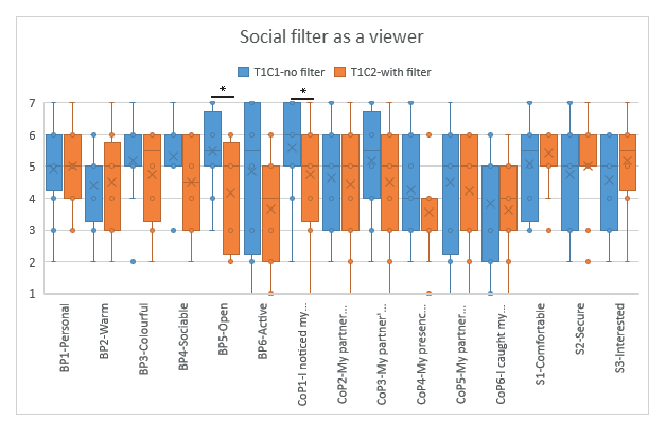
\includegraphics[width=.8\linewidth]{images/frontier18/images-03.eps}
\caption{Results of social filter as viewer. *= statistically significant}\label{fig:frontier18:result-filter-viewer}
\end{center}
\end{figure}

\begin{figure}
\begin{center}
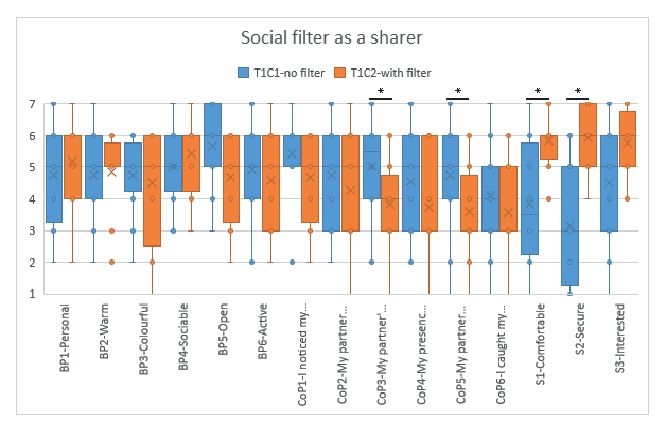
\includegraphics[width=.8\linewidth]{images/frontier18/images-04.eps}
\caption{Results of social filter as sharer. *= statistically significant}\label{fig:frontier18:result-filter-sharer}
\end{center}
\end{figure}



\begin{figure}
\begin{center}
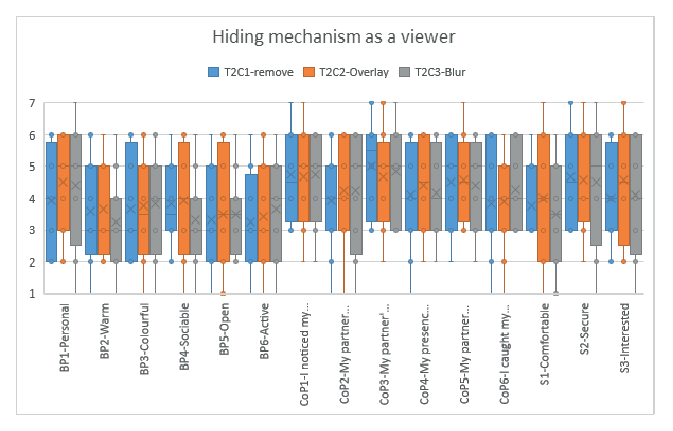
\includegraphics[width=.9\linewidth]{images/frontier18/images-05.eps}
\caption{Results of hiding mechanism as viewer.}\label{fig:frontier18:result-hiding-viewer}
\end{center}
\end{figure}

\begin{figure}
\begin{center}
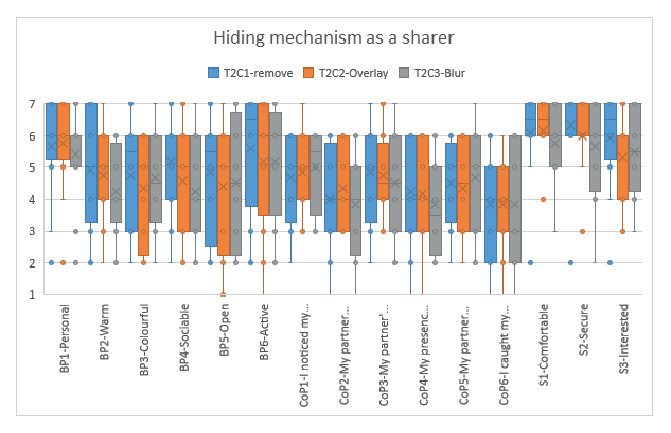
\includegraphics[width=.9\linewidth]{images/frontier18/images-06.eps}
\caption{Results of hiding mechanism as sharer.}\label{fig:frontier18:result-hiding-sharer}
\end{center}
\end{figure}

\begin{figure}
\begin{center}
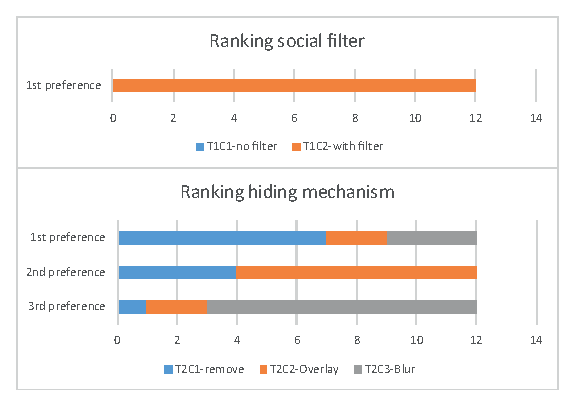
\includegraphics[width=.8\linewidth]{images/frontier18/images-07.eps}
\caption{Results of ranking conditions.}\label{fig:frontier18:result-ranking}
\end{center}
\end{figure}
